\documentclass[12pt,pdf,hyperref={unicode}]{beamer}
%\usetheme{boxes}
\beamertemplatenavigationsymbolsempty
\setbeamertemplate{footline}[page number]
% Set it for the internal PhD thesis defence to reduce number of slides
%\setbeamersize{text margin left=0.5em, text margin right=0.5em}

\usepackage[utf8]{inputenc}
%\usepackage[english, russian]{babel}
\usepackage{bm}
\usepackage{multirow}
\usepackage{ragged2e}
\usepackage{indentfirst}
\usepackage{multicol}
\usepackage{subfig}
\usepackage{amsmath,amssymb}
\usepackage{enumerate}
\usepackage{mathtools}
\usepackage{comment}
\usepackage[all]{xy}
\usepackage{tikz}
\usetikzlibrary{positioning,arrows}
\tikzstyle{name} = [parameters]
\definecolor{name}{rgb}{0.5,0.5,0.5}

%\usepackage{caption}
%\captionsetup{skip=0pt,belowskip=0pt}

%\newtheorem{theorem}{Theorem}
%\newtheorem{statement}{Statement}
%\newtheorem{definition}{Definition}

% colors
\definecolor{darkgreen}{rgb}{0.0, 0.2, 0.13}
\definecolor{darkcyan}{rgb}{0.0, 0.55, 0.55}
%\AtBeginEnvironment{figure}{\setcounter{subfigure}{0}}
%\captionsetup[subfloat]{labelformat=empty}

%----------------------------------------------------------------------------------------------------------

\title{ Put the title of your thesis \\ here}
%\author{Name Surname}
%\institute[]{}
%\date{2024}

%---------------------------------------------------------------------------------------------------------
\begin{document}
%\begin{frame}
%\titlepage
%\end{frame}
\setcounter{page}{2}%remove here for the title
%----------------------------------------------------------------------------------------------------------
%\section{Please do not use sectioning in the presentations}
\begin{frame}{Oxide identification by curve of gas dynamics}
\small{The analysis of oxide inclusions in metals is an important task in metallurgy, since different types of inclusions affect the properties of the metal in different ways.}
\begin{block}{The problem}
\small{To develop a method for determining the rate of CO release from oxide inclusions in a sample during Fractional Gas Analysis and the sample composition.}
\end{block}
\begin{block}{The method for metal oxide spectrum identification from non-isothermal gas dynamics}
The idea of method is using a neural network from the DeepXDE package that takes into account physical information.
\end{block}
\begin{block}{The solution}
\begin{enumerate}[1)]
\item The required method has been developed.
\item The method has been tested on 2 types of bearing steel.
\end{enumerate}
\end{block}
\end{frame}
%----------------------------------------------------------------------------------------------------------
\begin{frame}{The illustration of the method`s%
\footnote{\textit{Grigorovitch K. V., Krasovskii P. V., Krylov A. S.}  Fractional Gas Analysis-Basic Principles and Application in Steel Quality, 1999.} results}

\begin{enumerate}[1)]
    \item \small{The first figure shows an example of a hologram obtained as a result of fractional gas analysis. This is a graph of the dependence of the rate of CO release on temperature. }
    \item \small{The second graph shows the result of the method  on the SHX-15. These are the predicted curves of the CO release rate, showing what inclusions there are in the composition of the metal.}
\end{enumerate}
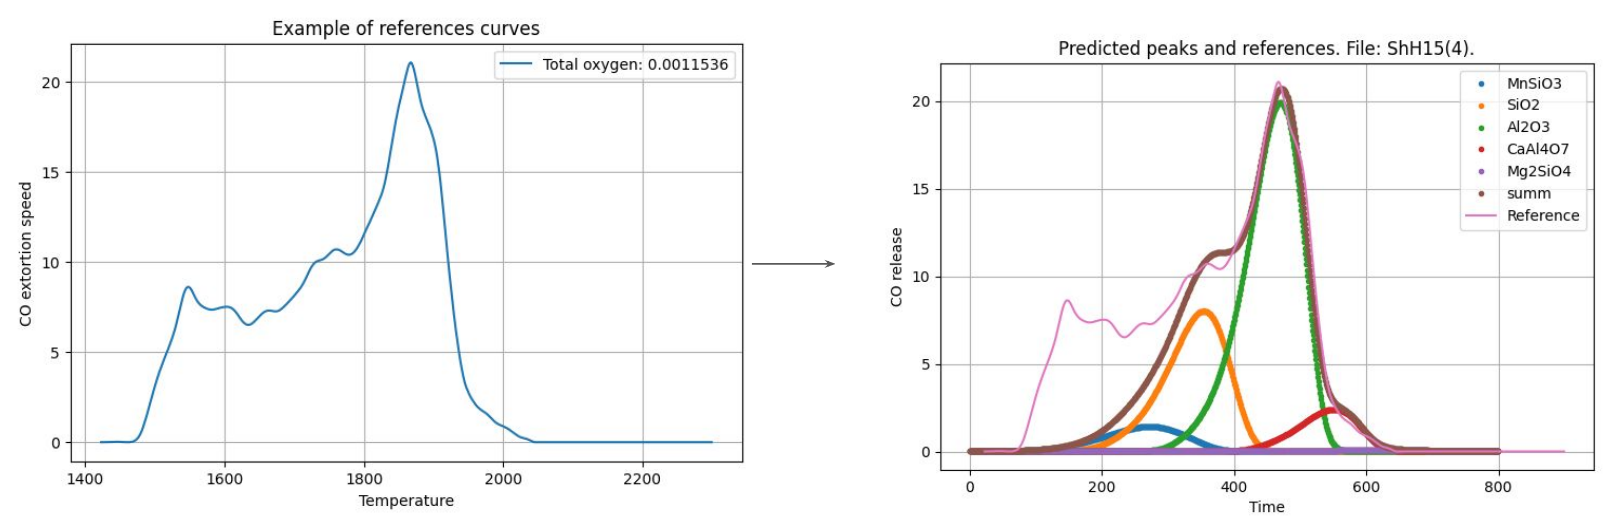
\includegraphics[width=1\textwidth]{graf-Step-3-fig.png}
\bigskip
\end{frame}
\end{document}